\subsection{Comparison with generative baselines}\label{sec:main-comparison}
Figure~\ref{fig:main-generators} compares raw outputs from LatentSpring, Gaussian-source FM, EDM, and GAGA on the same compositions. The latter three are evaluated without LatentSpring's recovery training or endpoint corrections.

\begin{figure}[!htbp]\centering
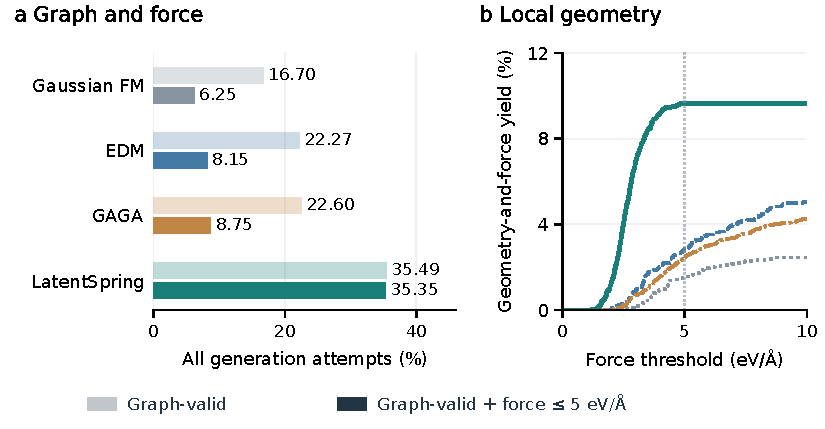
\includegraphics[width=\linewidth]{../research/figures/final_complete_v1/figures/main_comparison.pdf}
\caption{Generation on 64 unseen compositions. (a) Paired horizontal bars show graph validity (pale) and graph-and-force yield (solid) at a force-RMS threshold of 5 eV/\AA. (b) Geometry-and-force yield versus force threshold, with a vertical reference at 5 eV/\AA. Method colors match across panels. Gaussian FM and EDM have two fits and 2,048 outputs each; GAGA and LatentSpring have five fits and 5,120 outputs. All rates include every attempt, without hydrogen readout.}\label{fig:main-generators}
\end{figure}

LatentSpring achieves 35.49\% graph validity and 35.35\% graph-and-force yield. Joint yields for GAGA, EDM, and Gaussian FM are 8.75\%, 8.15\%, and 6.25\%, giving gains of 26.60, 27.20, and 29.10 percentage points. Under the stricter geometry-and-force criterion, LatentSpring reaches 9.63\%, compared with 2.40\%, 2.83\%, and 1.51\%, respectively.

Geometric refinement raises the five-fit geometry-and-force yield from 4.43\% for the initial force-corrected FM to 9.63\%. All three additional fits improve, with a mean gain of 5.08 points and a crossed fit/composition 95\% interval of $[3.09,7.52]$. In the two-fit control, the complete method reaches 10.25\%, compared with 5.76\% for unperturbed endpoint continuation with matched backbone updates: a 4.49-point gain, with crossed interval $[2.44,6.45]$. The control tests the complete refinement procedure, including its geometric head (Appendix~\ref{app:geometric-recovery}).

On the complementary 12-composition common-element organic panel, geometry-and-force yield is 35.42\% for LatentSpring, 20.57\% for the initial force-corrected FM, 17.71\% for GAGA, 14.84\% for EDM, and 16.41\% for Gaussian FM. The 14.84-point improvement over the initial FM has crossed interval $[7.81,25.52]$. Appendix~\ref{app:chemical-geometry} reports the panel selection, all 384 attempts per method, geometric checks, and charge-assignment diagnostics.
